% =============================================================================
% LaTeX Workshop Slide Deck, Northeastern University Wireless Club
% =============================================================================

% =============================================================================
% Beamer Theme Customizations
% =============================================================================
\documentclass[x11names]{beamer}                            % Global option [x11names] avoids xcolor clash
\usetheme{Madrid}
\usecolortheme{beaver}
\setbeamertemplate{navigation symbols}{}                    % Hides navigation buttons at bottom-right
\setbeamercovered{transparent}                              % Make hidden items (e.g., \onslide, \only) semi-transparent
\setbeamercolor{section in head/foot}{bg=gray!60, fg=black} % Set a darker gray-ish color for the "section in head/foot".
                                                            % This is the bottom-right footer column used for displaying 
                                                            % the version (Git commit hash) and the page numbering.

															
% =============================================================================
% Packages
% =============================================================================
\usepackage{graphicx}   % For including images (e.g., QR codes)
\usepackage{hyperref}   % For clickable hyperlinks
\usepackage{xcolor}     % For defining custom colors (e.g., the urlcolor)
\usepackage{iexec}      % Run command line (used for Git hash in versioning)
\usepackage{tcolorbox}  % For colored boxes
\usepackage{qrcode}     % For generating QR codes
\usepackage[utf8]{inputenc}
\usepackage{mdframed}   % For framed environments
\usepackage{minted}     % For syntax-highlighted code blocks
\usepackage{tikz}       % For drawing (used in mdframed titles)
\usepackage{lastpage}   % For referencing the total number of pages, used in footer as \pageref{LastPage}
                        % requires compiling the document twice to resolve the total page count correctly

\usetikzlibrary{automata, positioning, arrows}
\tikzset{
	->,
	node distance=3cm,
	every state/.style={thick, fill=gray!10},
	initial text=$ $,
}

% =============================================================================
% Versioning (Git commit hash for version info in footer)
% =============================================================================
\newcommand{\gitAbbrevHash}{\iexec{git rev-parse --short HEAD}}

% =============================================================================
% Custom Environments
% =============================================================================
\newenvironment{question}[1][]{
  \ifstrempty{#1}{}{
    \mdfsetup{
      frametitle={
        \tikz[baseline=(current bounding box.east),outer sep=0pt]
        \node[anchor=east,rectangle,fill=gray!30]{#1};
      }}
  }
  \mdfsetup{
    innertopmargin=10pt,
    linecolor=gray!30,
    linewidth=2pt,
    topline=true,
    frametitleaboveskip=\dimexpr - \ht\strutbox\relax
  }
  \begin{mdframed}
}{\end{mdframed}}

% =============================================================================
% Custom Color Definitions
% =============================================================================
\definecolor{nuRed}{HTML}{C8102E}  % Northeastern University primary brand red

% =============================================================================
% Hyperlink Configuration
% =============================================================================
\hypersetup{
  colorlinks=true,
  linkcolor=blue,
  urlcolor=nuRed
}

% =============================================================================
% Footer Configuration
% =============================================================================
% Customizes the footer to display organization, workshop name, semester, version, and page number
\setbeamertemplate{footline}{%
  \leavevmode%
  \hbox{
    % Left: Organization Name
    \begin{beamercolorbox}[wd=.35\paperwidth,ht=2.25ex,dp=1ex,leftskip=.3cm]{author in head/foot}%
      Northeastern University Wireless Club%
    \end{beamercolorbox}%
    % Center: Workshop Name
    \begin{beamercolorbox}[wd=.20\paperwidth,ht=2.25ex,dp=1ex,center]{title in head/foot}%
      Intro to Git Workshop%
    \end{beamercolorbox}%
    % Center: Semester Information
    \begin{beamercolorbox}[wd=.15\paperwidth,ht=2.25ex,dp=1ex,center]{date in head/foot}%
      Fall 2025%
    \end{beamercolorbox}%
    % Right: Version (Git commit hash) and Page Number
    \begin{beamercolorbox}[wd=.30\paperwidth,ht=2.25ex,dp=1ex,leftskip=.3cm, rightskip=.3cm plus1fil]{section in head/foot}%
      Version: \gitAbbrevHash{} \hspace{1em} \insertpagenumber/\inserttotalframenumber%
    \end{beamercolorbox}}%
  \vskip0pt%
}

% =============================================================================
% Title Page Information 
% =============================================================================
\title{Intro to Git Workshop}
\subtitle{Fall 2025}
\author{
  Northeastern University Wireless Club - W1KBN \\
  {\small Muhammad Elarbi, Robert Halpern, Tyler Von Pervieux}
  }
\date{November 10, 2025}

\begin{document}

% =============================================================================
% Slide: Title Page + Sign-In with QR Code
% =============================================================================
\begin{frame}
  \titlepage
  \vspace{-1cm}
  \begin{center}
    \textbf{Sign in Here:} \\ 
    \qrcode{https://forms.gle/EukxnYUPSvckBFsg7} \\
    {\small \href{https://nuwireless.org/signin}{nuwireless.org/signin}}
  \end{center}
\end{frame}

% =============================================================================
% Slide: About Us 
% =============================================================================
\begin{frame}
	\begin{tcolorbox}[colframe=black, colback=blue!10, title=About, center title]
	\begin{itemize}
		\item Regular Meetings: Thursdays, 7 PM @ Hayden Hall, Room 503
		\item Workshops: Mondays, 7:10 PM @ Forsyth Building, Room 236
	\end{itemize}        
	\end{tcolorbox}
	\begin{center}
		\Large Thank you for a great workshop season! 
	\end{center}
\end{frame}


\begin{frame}
	\frametitle{Intro: Workshop Structure}
	\centering \textbf{Structure:}
	\begin{enumerate}
		\setlength\itemsep{1em}
		\item Background: how does \texttt{Git} work?
		\item Example: managing homework
		\item Hands-on: solve \texttt{Git} `puzzles' in browser
	\end{enumerate}
	\vfill
	\centering \textbf{General:}
	\begin{itemize}
		\setlength\itemsep{1em}
		\item Ask questions!
		      (want to know more? something isn't clear?)
		\item Reach out: \url{neuwireless.slack.com}
	\end{itemize}
\end{frame}

\begin{frame}
	\frametitle{Intro: Teaching \texttt{Git}}
	\begin{figure}
		
\includegraphics[height=\textheight-25mm]{assets/xkcd-git-comic.png}
		\caption{XKCD 1597 `Git' --- CC BY-NC 2.5}
	\end{figure}
\end{frame}

\begin{frame}
	\frametitle{Background: What is \texttt{Git}?}
	\vfill
	\begin{figure}
		
\includegraphics[height=15mm]{assets/git-logo.png}
		\caption{Git Logo --- CC BY 3.0}
	\end{figure}
	\vfill
	\begin{itemize}
		\item broadly; \emph{a tool used to track changes to files and folders.}
		\item facilitates collaboration on software projects
		\item captures `snapshots' of a project
		\item maintains metadata
		      \begin{itemize}
			      \item what was changed
			      \item who was it changed by
			      \item when was it changed
			      \item messages associated with changes
		      \end{itemize}
	\end{itemize}
	\vfill
\end{frame}

\begin{frame}
	\frametitle{Background: What is \texttt{Git} used for?}
	\vfill
	\centering \textbf{Group Applications (Industry, co-op)}
	\begin{itemize}
		\item large software projects
		\item resolve conflicts when multiple people are editing the same things
		\item who wrote this!?
	\end{itemize}
	\vfill
	\centering \textbf{Personal Applications}
	\begin{itemize}
		\item ``I swear this worked 10 minutes ago\ldots''
		\item find what broke something and when
		\item separate tasks; work on bug fixing is isolated from work on new feature
		\item can use for class work!
	\end{itemize}
	\vfill
\end{frame}

\begin{frame}
	\frametitle{Background: Big Idea of \texttt{Git}}
	\begin{question}[QUESTION: Intuition]
		based on this description of what \texttt{Git} does, can you imagine how you would go about making these `snapshots' manually?
	\end{question}
	\vfill
	\begin{figure}
		
\includegraphics[width=3cm]{assets/git-snapshot.png}
	\end{figure}
\end{frame}

\begin{frame}
	\frametitle{Background: Big Idea of \texttt{Git}}
	\begin{figure}
		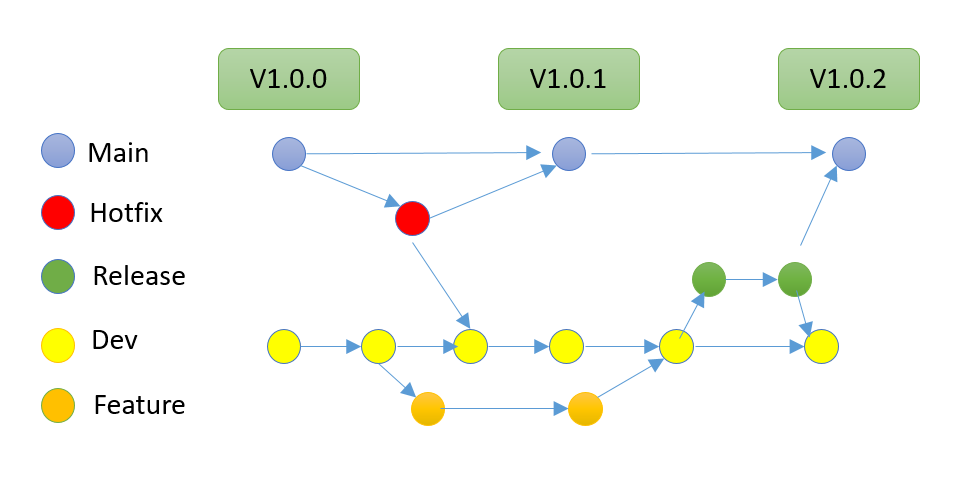
\includegraphics[width=\linewidth]{assets/branching.png}
	\end{figure}
\end{frame}

\begin{frame}
	\frametitle{Example: Managing Local Files}
	\vfill
	\begin{question}[EXAMPLE: Homework Files]
		\begin{enumerate}
			\item \emph{Init}: make a file
			\item \emph{Add/Commit}: save file
			\item \emph{Branch/Checkout}: two new features
			\item \emph{Merge}: combine those new features
			\item \emph{Restore/Checkout}: restore save
		\end{enumerate}
	\end{question}
	\vfill
\end{frame}

\begin{frame} \frametitle{Background: \texttt{Git} vs. \texttt{GitHub}?}
	\centering \textbf{What's the difference between \texttt{Git} and \texttt{GitHub}?}
	\vfill
	\begin{columns}[t]
		\begin{column}{0.33\textwidth}
			\centering \textbf{Git}
			\begin{itemize}
				\item a program running on your computer
				\item used to manage repositories
				\item open-source and independent of GitHub
			\end{itemize}
		\end{column}
		\begin{column}{0.67\textwidth}
			\centering \textbf{GitHub}
			\begin{itemize}
				\item a company
				\item centralized location to store git repositories (git server)
				\item alternatives: GitLab, SourceHut, BitBucket, Gitea, self hosting, \ldots
				\item additional project management utilities
				\item CI, CD, hosting, \ldots
			\end{itemize}
		\end{column}
	\end{columns}
\end{frame}

\begin{frame}
	\frametitle{Practical Git}
	\vfill
	\begin{question}[EXAMPLE: Create new repository]
		\begin{enumerate}
			\item Initialize \quad \texttt{git init}
			\item Make an initial commit \quad \texttt{git commit --allow-empty}
			\item Add a remote \quad \texttt{git remote add ...}
		\end{enumerate}
	\end{question}
	\vfill
	\begin{question}[EXAMPLE: Commit all current changes]
		\begin{enumerate}
			\item Prepare files for commit \quad \texttt{git add -A}
			\item Check your changes \quad \texttt{git diff --staged}
			\item Create a commit \quad \texttt{git commit -m "my changes"}
			\item Push to remote \quad \texttt{git push}
		\end{enumerate}
	\end{question}
	\vfill
\end{frame}

\begin{frame}
	\frametitle{Git Tips}
	\centering \textbf{}
	\begin{itemize}
		\item Make an empty initial commit
		\item Make small, incremental commits
		\item Use \texttt{git commit --amend}, if you messed up
		\item You can wait to \texttt{git push}
		\item (Software Only) Do not commit binaries, build outputs
	\end{itemize}
\end{frame}

\begin{frame}
	\frametitle{See Also}
	\centering \textbf{General}
	\begin{itemize}
		\setlength\itemsep{1em}
		\item \href{https://missing.csail.mit.edu/2020/version-control/}{MIT Missing Semester Lecture 6: Version Control (Git)}
		\item \href{https://tbaggery.com/2008/04/19/a-note-about-git-commit-messages.html}{Tim Pope: A Note About Git Commit Messages}
		\item \href{https://wyag.thb.lt/}{Implement git from scratch in Python}
		\item
		      \href{https://docs.github.com/en/free-pro-team@latest/github/collaborating-with-issues-and-pull-requests/about-pull-requests}{How to contribute to code on GitHub}
	\end{itemize}
	\vfill
	\centering \textbf{Git Documentation}
	\begin{itemize}
		\item \href{https://git-scm.com/docs/git-config}{Git configuration documentation}
		\item \href{https://git-scm.com/docs/gitignore}{\texttt{.gitignore} documentation}
	\end{itemize}
\end{frame}

\begin{frame}
	\frametitle{Hands-On With \texttt{git}}
	\centering
	\large{\url{https://learngitbranching.js.org/}}
\end{frame}

% -----------------------------------------------------------------------------
% Slide: Contact Information
% -----------------------------------------------------------------------------
\begin{frame}
    \frametitle{Contact Us}
    \begin{itemize}
        \item Questions? Feel free to reach out!
        \item Workshop Team Emails: \\
        \{\href{mailto:elarbi.m@northeastern.edu}{elarbi.m}, 
        \href{mailto:halpern.ro@northeastern.edu}{halpern.ro}, 
        \href{mailto:vonpervieux.t@northeastern.edu}{vonpervieux.t}\}[at]northeastern[d0t]edu
        \item General Workshop Email: \href{mailto:workshops@nuwireless.org}{workshops}[at]nuwireless[d0t]org
        \item Website: \url{https://nuwireless.org/}
        \item Location: Hayden Hall, Room 503
    \end{itemize}
    \vspace{1cm}
    \begin{flushright}
        \footnotesize{© 2025 Northeastern Wireless Club} \\
        \footnotesize{Design: \href{https://melarbi.com}{Muhammad Elarbi}, based on \LaTeX\ Beamer}\\
    \end{flushright}
\end{frame}

\end{document}
